\documentclass{beamer}

\mode<presentation> {

%\usetheme{default}
%\usetheme{AnnArbor}
%\usetheme{Antibes}
%\usetheme{Bergen}
%\usetheme{Berkeley}
%\usetheme{Berlin}
%\usetheme{Boadilla}
%\usetheme{CambridgeUS}
%\usetheme{Copenhagen}
%\usetheme{Darmstadt}
%\usetheme{Dresden}
%\usetheme{Frankfurt}
%\usetheme{Goettingen}
%\usetheme{Hannover}
%\usetheme{Ilmenau}
%\usetheme{JuanLesPins}
%\usetheme{Luebeck}
\usetheme{Madrid}
%\usetheme{Malmoe}
%\usetheme{Marburg}
%\usetheme{Montpellier}
%\usetheme{PaloAlto}
%\usetheme{Pittsburgh}
%\usetheme{Rochester}
%\usetheme{Singapore}
%\usetheme{Szeged}
%\usetheme{Warsaw}


%\usecolortheme{albatross}
%\usecolortheme{beaver}
%\usecolortheme{beetle}
%\usecolortheme{crane}
%\usecolortheme{dolphin}
%\usecolortheme{dove}
%\usecolortheme{fly}
%\usecolortheme{lily}
%\usecolortheme{orchid}
%\usecolortheme{rose}
%\usecolortheme{seagull}
%\usecolortheme{seahorse}
%\usecolortheme{whale}
%\usecolortheme{wolverine}

%\setbeamertemplate{footline} % To remove the footer line in all slides uncomment this line
%\setbeamertemplate{footline}[page number] % To replace the footer line in all slides with a simple slide count uncomment this line

%\setbeamertemplate{navigation symbols}{} % To remove the navigation symbols from the bottom of all slides uncomment this line
}

\usepackage{graphicx} % Allows including images
\usepackage{booktabs} % Allows the use of \toprule, \midrule and \bottomrule in tables
\usepackage{amsfonts}
\usepackage{mathrsfs, bbold}
\usepackage{amsmath,amssymb,graphicx}
\usepackage{mathtools} % gather
\usepackage[export]{adjustbox} % right-aligned graphics


% sectioning stuff
% Add support for \subsubsectionpage
\def\subsubsectionname{\translate{Subsubsection}}
\def\insertsubsubsectionnumber{\arabic{subsubsection}}
\setbeamertemplate{subsubsection page}
{
  \begin{centering}
    {\usebeamerfont{subsubsection name}\usebeamercolor[fg]{subsubsection name}\subsubsectionname~\insertsubsubsectionnumber}
    \vskip1em\par
    \begin{beamercolorbox}[sep=4pt,center]{part title}
      \usebeamerfont{subsubsection title}\insertsubsubsection\par
    \end{beamercolorbox}
  \end{centering}
}
\def\subsubsectionpage{\usebeamertemplate*{subsubsection page}}

\AtBeginSection{\frame{\sectionpage}}
\AtBeginSubsection{\frame{\subsectionpage}}
\AtBeginSubsubsection{\frame{\subsubsectionpage}}


%----------------------------------------------------------------------------------------
%	TITLE PAGE
%----------------------------------------------------------------------------------------

\title["11"]{11: Basics of Markov chain Monte Carlo Simulation}

\author{Taylor} 
\institute[UVA] 
{
University of Virginia \\
\medskip
\textit{} 
}
\date{} 

\begin{document}
%----------------------------------------------------------------------------------------

\begin{frame}
\titlepage 
\end{frame}

%----------------------------------------------------------------------------------------
\section{General Ideas}
\begin{frame}
\frametitle{Introduction}

In this section, we discuss {\bf Markov chain Monte Carlo} techniques, which all produce \underline{correlated} draws from the posterior of interest.
\newline

Compared with chapter 12, this chapter mostly seeks to build intuition and mention key ideas.


\end{frame}

%----------------------------------------------------------------------------------------
\begin{frame}
\frametitle{Overview}

Even though we might not even have a time series model, we construct a Markov chain 
$$
\theta^1, \theta^2, \ldots, \theta^N
$$
Even though these draws are correlated, they are all {\bf marginally} distributed according to the posterior 
$$
p(\theta \mid y),
$$
and it is still legitimate to estimate expectations with sample means:
$$
E[h(\theta) \mid y] \approx  \frac{1}{N}\sum_{i=1}^N h(\theta^i).
$$
\end{frame}

%----------------------------------------------------------------------------------------
\begin{frame}
\frametitle{Typical MCMC Output}

A 2-parameter model:
\begin{center}
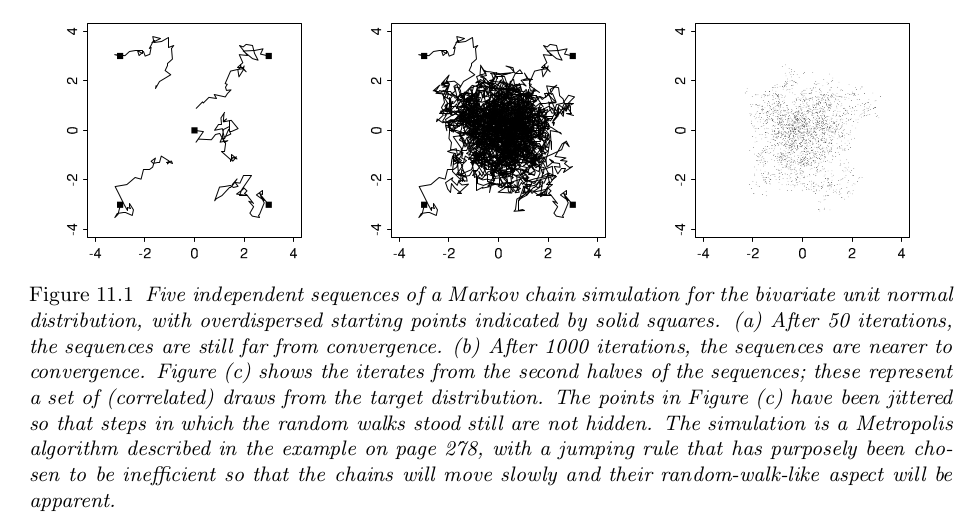
\includegraphics[width=120mm]{fig11.png}
\end{center}

\end{frame}




%----------------------------------------------------------------------------------------
\begin{frame}
\frametitle{Typical MCMC Output}

Another 2-parameter model:

\begin{center}
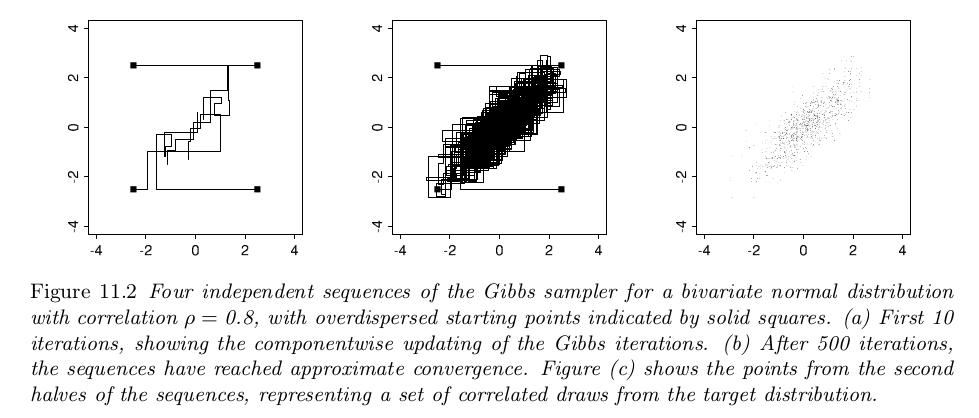
\includegraphics[width=120mm]{gibbs.png}
\end{center}

\end{frame}




%----------------------------------------------------------------------------------------
\begin{frame}
\frametitle{Typical MCMC Output}

A 6-parameter model from: \url{https://academic.oup.com/jfec/article/14/2/278/1751519}

\begin{center}
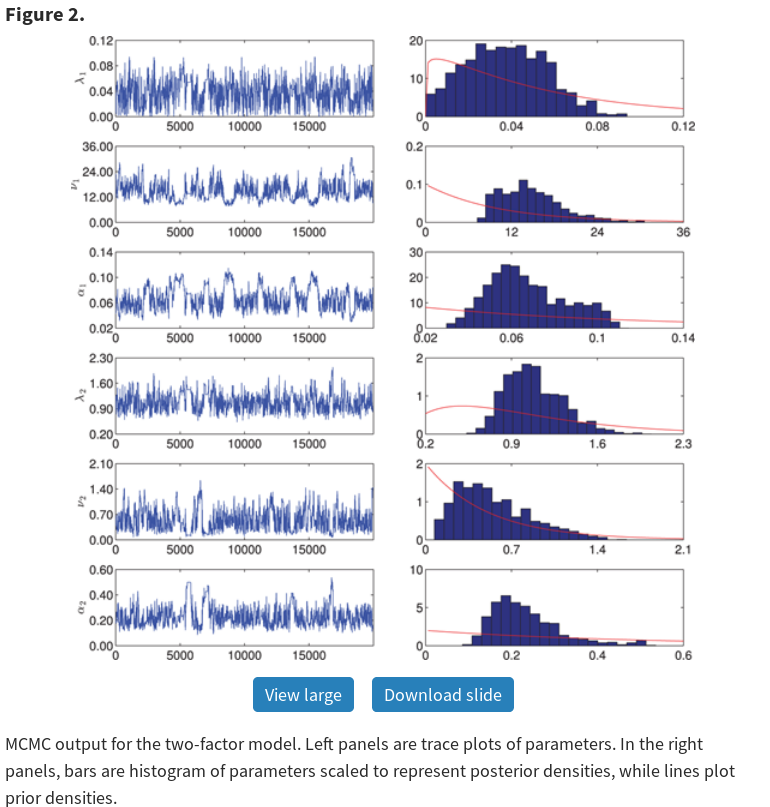
\includegraphics[width=70mm]{trace_hist.png}
\end{center}

\end{frame}

%----------------------------------------------------------------------------------------
\begin{frame}
\frametitle{Variance of our Estimator}

Let $\sigma^2 = \operatorname{Var}[h(\theta^i)]$, $\rho(h) = \operatorname{Corr}\left(  h(\theta^i), h(\theta^{h+i}) \right)$. If all of these variances are finite, then
\begin{align*}
N \operatorname{Var}\left[ \frac{1}{N}\sum_{i=1}^N h(\theta^i) \right] &= N\operatorname{Cov}\left( \frac{1}{N}\sum_{i=1}^N h(\theta^i),\frac{1}{N}\sum_{j=1}^N h(\theta^j) \right) \tag{defn.} \\
&= \frac{1}{N} \sum_{i=1}^N\sum_{j=1}^N\operatorname{Cov}\left(  h(\theta^i), h(\theta^i) \right) \tag{bilinearity} \\
&= \sigma^2 \left\{ 1 + 2\sum_{h=1}^N \frac{N - h}{N} \rho(h)\right\}  \tag{count diagonally} \\
&\to \sigma^2 \underbrace{\left\{ 1 + 2\sum_{h=1}^{\infty}  \rho(h)\right\}}_{\text{correlation is bad!}} 
\end{align*}



\end{frame}


%----------------------------------------------------------------------------------------
\begin{frame}
\frametitle{Typical MCMC Output}

Assessing the integrated autocorrelation with acf plots:
\begin{center}
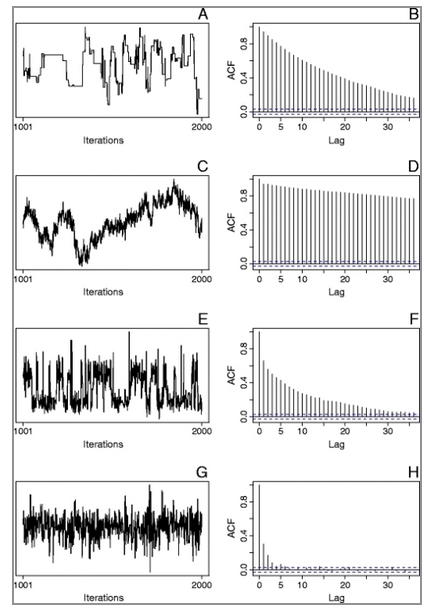
\includegraphics[width=40mm]{autocorr.png}
\end{center}
bad, bad, less bad, good.
\url{https://openi.nlm.nih.gov/detailedresult?img=PMC3218285_13428_2011_114_Fig10_HTML&req=4}

\end{frame}

%----------------------------------------------------------------------------------------
\begin{frame}
\frametitle{Another issue: has there been convergence?}

The previous expression assumes each draw is distributed according to the posterior. 
\newline

If we start the chain far away from the mode, how long until it converges? How can we be sure it has converged? If you don't run your algorithm for long enough, your answer will be very wrong.
\newline
\pause

Trace plots help. We also have convergence diagnostics.
\newline

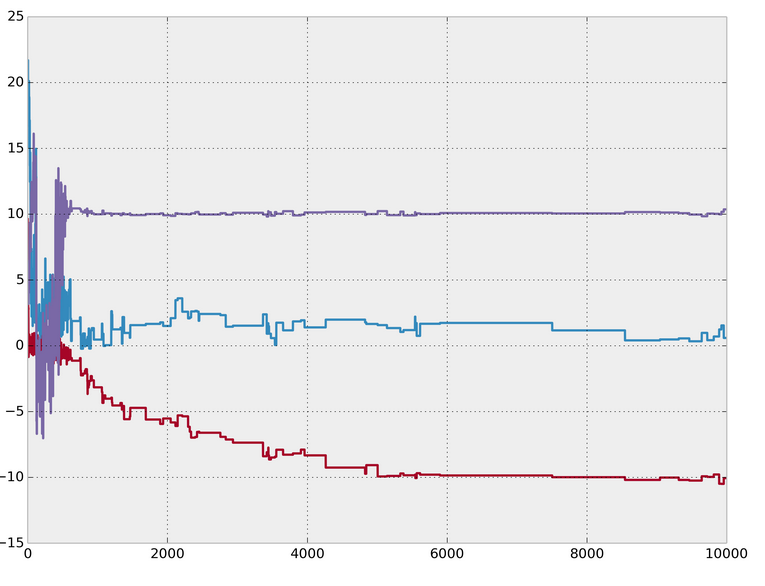
\includegraphics[width=40mm]{convergence.png} You could throw away $6000$ iterations as a {\bf burn in} or {\bf warm-up}.

\end{frame}

%----------------------------------------------------------------------------------------
\begin{frame}
\frametitle{Assessing convergence for scalars $\psi_{i,j}$ using $\hat{R}$}

Run $m$ chains for $n$ iterations, $i=1,\ldots,n$ and $j=1\ldots,m$.
\begin{align*}
\bar{\psi}_{\cdot \cdot} &= \frac{1}{mn}\sum_{i=1}^n\sum_{j=1}^m \psi_{ij} \tag{overall average} \\
\bar{\psi}_{\cdot j} &= \frac{1}{n}\sum_{i=1}^n \psi_{ij} \tag{chain average} \\
s^2_j &= \frac{1}{n-1}\sum_{i=1}^n (\psi_{ij}-\bar{\psi}_{\cdot j})^2 \tag{chain sd} \\
W &= \frac{1}{m} s^2_j \tag{within-sequence variance} \\
B &= \frac{n}{m-1} \sum_{j=1}^m (\bar{\psi}_{\cdot j} - \bar{\psi}_{\cdot \cdot})^2\\
\widehat{\text{var}}^{+}(\psi \mid y) =\frac{n-1}{n}W &+ \frac{1}{n}B \hspace{10mm} \hat{R} = \sqrt{\widehat{\text{var}}^{+}(\psi \mid y) / W}.
\end{align*}

Split each chain into two, after discarding a burn-in/warm-up.
%On page 284
\end{frame}


%----------------------------------------------------------------------------------------
\section{Description of Algorithms}
\begin{frame}
\frametitle{Metropolis-Hastings algorithm}

At iteration $t-1$ you have $\theta^{t-1}$. Propose $\theta^* \sim q(\theta \mid \theta^{t-1})$, and accept this draw with probability 
$$
a(\theta^{t-1}, \theta^*) = \min\left\{1, \frac{p(\theta^* \mid y)q(\theta^{t-1} \mid \theta^*) }{p(\theta^{t-1} \mid y) q(\theta^* \mid \theta^{t-1}) }\right\}.
$$
If you accept, $\theta^t \overset{\text{set}}{=} \theta^*$. Otherwise, $\theta^t \overset{\text{set}}{=} \theta^{t-1}$. 
\newline

{\it Many} algorithms are a special case of this one.

\end{frame}

%----------------------------------------------------------------------------------------
\begin{frame}
\frametitle{Metropolis-Hastings algorithm}

Why it's widely-applicable:
\begin{align*}
a(\theta^{t-1}, \theta^*) &= \min\left\{1, \frac{p(\theta^* \mid y)q(\theta^{t-1} \mid \theta^*) }{p(\theta^{t-1} \mid y) q(\theta^* \mid \theta^{t-1}) }\right\} \\
&= \min\left\{1, \frac{p(\theta^*, y)/p(y)q(\theta^{t-1} \mid \theta^*) }{p(\theta^{t-1}, y)/p(y) q(\theta^* \mid \theta^{t-1}) }\right\} \\
&= \min\left\{1, \frac{p(y \mid \theta^*) p(\theta^*)q(\theta^{t-1} \mid \theta^*) }{p(y \mid \theta^{t-1}) p(\theta^{t-1}) q(\theta^* \mid \theta^{t-1}) }\right\}.
\end{align*}
Don't need to know the normalizing constant/marginal likelihood/evidence!

\end{frame}
%----------------------------------------------------------------------------------------
\begin{frame}
\frametitle{Metropolis-Hastings algorithm}

$$
a(\theta^{t-1}, \theta^*) = \min\left\{1, \frac{p(\theta^* \mid y)q(\theta^{t-1} \mid \theta^*) }{p(\theta^{t-1} \mid y) q(\theta^* \mid \theta^{t-1}) }\right\}.
$$

\begin{enumerate}
\item When is $a(\theta^{t-1}, \theta^*)$ nearly $1$?
\item When is $a(\theta^{t-1}, \theta^*)$ nearly $0$?
\item How should we pick $q(\theta^* \mid \theta^{t-1})$?
\item What is the ideal $q(\theta^* \mid \theta^{t-1})$?
\item What if $q(\theta^* \mid \theta^{t-1})$ is too peaked?
\item What if $q(\theta^* \mid \theta^{t-1})$ is too diffuse?
\end{enumerate}


\end{frame}
%----------------------------------------------------------------------------------------
\begin{frame}
\frametitle{Metropolis-Hastings algorithm}

Let's pick $q(\theta \mid \theta^{t-1}) = \text{Normal}(\theta^{t-1}, \sigma^2 {\bf I} )$
\newline

\url{https://chi-feng.github.io/mcmc-demo/app.html\#RandomWalkMH,banana}
\end{frame}



%----------------------------------------------------------------------------------------
\begin{frame}
\frametitle{Independent Metropolis Hastings}

If $q(\theta \mid \theta^{t-1}) = q(\theta)$ (i.e. propose independently of past values), then you have the {\bf Independent Metropolis Hastings} algorithm, which has acceptance probabilities
$$
a(\theta^{t-1}, \theta^*) = \min\left\{1, \frac{p(\theta^* \mid y)q(\theta^{t-1} ) }{p(\theta^{t-1} \mid y) q(\theta^* ) } \right\}.
$$

The proposals are iid, but the chain is Markovian!

\end{frame}

%----------------------------------------------------------------------------------------
\begin{frame}
\frametitle{Metropolis algorithm}

If $q(\theta^* \mid \theta^{t-1}) = q(\theta^{t-1} \mid \theta^*)$ (i.e. $q$ is {\bf symmetric}), the acceptance probability
$$
a(\theta^{t-1}, \theta^*) = \min\left\{1, \frac{p(\theta^* \mid y)q(\theta^{t-1} \mid \theta^*) }{p(\theta^{t-1} \mid y) q(\theta^* \mid \theta^{t-1}) }\right\}.
$$
becomes
$$
a(\theta^{t-1}, \theta^*) = \min\left\{1, \frac{p(\theta^* \mid y)}{p(\theta^{t-1} \mid y)  }\right\}.
$$
and they call this the {\bf Metropolis} algorithm (drop the ``Hastings").

\end{frame}

%----------------------------------------------------------------------------------------
\begin{frame}
\frametitle{The Gibbs Sampler}

Say there are two parameters: $\theta = (\theta_1, \theta_2)$. The {\bf Gibbs sampler} alternates between 
\begin{enumerate}
\item $\theta_1^t \sim p(\theta_1 \mid \theta_2^{t-1}, y)$
\item $\theta_2^t \sim p(\theta_2 \mid \theta_1^{t}, y)$
\end{enumerate}

If there are more parameters: $\theta = (\theta_1, \theta_2, \ldots, \theta_d)$. The Gibbs sampler alternates between 
\begin{enumerate}
\item $\theta_1^t \sim p(\theta_1 \mid \theta_{2:d}^{t-1}, y)$
\item $\theta_2^t \sim p(\theta_2 \mid \theta_1^t, \theta_{3:d}^{t-1}, y)$
\item $\vdots$
\item $\theta_d^t \sim p(\theta_d \mid \theta_{1:d-1}^{t}, y)$
\end{enumerate}

This is only possible if you can sample from the {\bf conditional posteriors} (i.e. need conditional conjugacy).

\end{frame}

%----------------------------------------------------------------------------------------
\begin{frame}
\frametitle{The Gibbs Sampler}

Example on page 277:
\begin{enumerate}
\item $\theta_1 \mid \theta_2, y \sim \text{Normal}(y_1 + \rho(\theta_2 - y_2), 1-\rho^2)$
\item $\theta_2 \mid \theta_1, y \sim \text{Normal}(y_2 + \rho(\theta_1 - y_1), 1-\rho^2)$
\end{enumerate}

\begin{center}
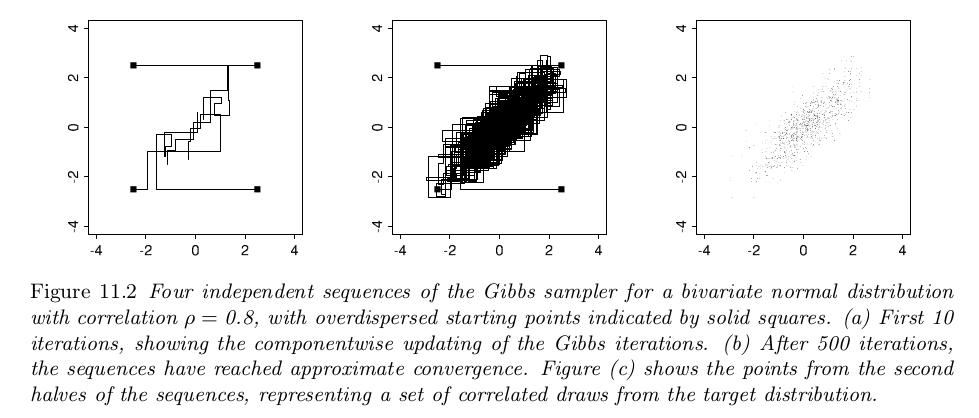
\includegraphics[width=80mm]{gibbs.png}
\end{center}


\end{frame}

%----------------------------------------------------------------------------------------
\section{A Closer Look}
\begin{frame}
\frametitle{Metropolis-Hastings algorithm}

Often $\theta^* \sim q(\theta \mid \theta^{t-1})$ is a density (continuous random variable), but the actual transition is not. 
\newline

We call the probability of rejecting/staying put: 
$$
r(\theta^{t-1}) = 1 - \int a(\theta^{t-1}, \theta^*)q(\theta^* \mid \theta^{t-1}) \text{d}\theta^* 
$$



\end{frame}



%----------------------------------------------------------------------------------------
\begin{frame}
\frametitle{Metropolis-Hastings algorithm}

The transition dynamics for a MH chain is usually written down as a {\bf kernel} 
\begin{align*}
P(\theta^t \in A \mid \theta^{t-1}) &= P(\theta^{t-1}, A) \\
&= r(\theta^{t-1})I(\theta^{t-1}, A) + \int_A a(\theta^{t-1}, \theta^*)q(\theta^* \mid \theta^{t-1}) \text{d}\theta^*
\end{align*}

\begin{enumerate}
\item it's more common for things to be written in a left-to-right format instead of a right-to-left
\item it's also more common for elements of the state space to be written with letters (e.g. $x$, $y$)
\end{enumerate}
We switch to left-to-right, x and y notation, and then we switch back later.



\end{frame}

%----------------------------------------------------------------------------------------
\begin{frame}
\frametitle{Metropolis-Hastings algorithm}

Call the target distribution $\pi$ (i.e. the posterior), and call our Markov transition kernel $P(x, A)$.
\newline

$\pi$ is the {\bf stationary distribution} for $P$ if
$$
\int \pi(x) P(x, A) \text{d}x = \pi(A).
$$
Sometimes this is written as $\pi P = \pi$




\end{frame}

%----------------------------------------------------------------------------------------
\begin{frame}
\frametitle{Metropolis-Hastings algorithm}

Call the target distribution $\pi$ (i.e. the posterior), and call our Markov transition kernel $P(x, A)$.
\newline

The Markov chain is {\bf reversible} if
$$
\int_A\int_B \pi(x) P(x, dy) \text{d}x = \int_B\int_A \pi(x) P(x, dy) \text{d}x.
$$
Being in $B$ and then $A$ has the same chances as being in $A$ and then $B$. 
\newline

This is the same thing as exchangeability! Think about when something like this wouldn't be true.

\end{frame}

%----------------------------------------------------------------------------------------
\begin{frame}
\frametitle{Metropolis-Hastings algorithm}

Call the target distribution $\pi$ (i.e. the posterior), and call our Markov transition kernel $P(x, A)$.
\newline

Reversibility implies stationarity. Just take $B = \mathsf{X}$ (the entire space):
$$
\int_A\int_B \pi(x) P(x, dy) \text{d}x = \int_B\int_A \pi(x) P(x, dy) \text{d}x.
$$

\end{frame}

%----------------------------------------------------------------------------------------
\begin{frame}
\frametitle{Why Everything ``Works"}

Virtually every MCMC we discuss has a ``law of large numbers." This is because every Markov chain we talk about is {\bf ergodic}, which means 
$$
\Vert P^n(x,A)- \pi(A) \Vert_{TV} \to 0 \hspace{10mm} \text{as } n \to \infty.
$$
This is convergence in total variation, which is stronger than convergence in distribution.
\newline

To calculate confidence intervals, you will need central limit theorems, which require stronger forms of ergodicity. These are more technical, and are outside the scope of this class.




\end{frame}


%----------------------------------------------------------------------------------------
\begin{frame}
\frametitle{Example: Hierarchical Normal Model}

\begin{enumerate}
\item $y_{ij} \sim \text{Normal}(\theta_j, \sigma^2)$
\item $\theta_j \sim \text{Normal}(\mu, \tau^2)$
\item $p(\mu) \sim \text{Normal}(60, 100)$
\item $p(\tau^2) = \text{Inverse-Gamma}(.001, .001)$
\item $p(\sigma^2) = \text{Inverse-Gamma}(.001, .001)$
\end{enumerate}

\end{frame}

%----------------------------------------------------------------------------------------
\begin{frame}
\frametitle{Example: Hierarchical Normal Model (MH)}

We either need to worry about constraints, or we can sample on a transformed space.
\newline

Let's sample on the transformed space. Be careful of the Jacobians. If $p(\sigma^2) \propto (\sigma^2)^{-.0001-1}\exp\left[- .0001 \sigma^{-2} \right]$, then
$$
p(\log \sigma) \propto (\sigma^2)^{-.0001}\exp\left[- .0001 \sigma^{-2} \right] .
$$
Also
$$
p(\log \tau) \propto (\tau^2)^{-.0001}\exp\left[- .0001 \tau^{-2} \right]
$$
%\item $\log p(\log \sigma) = c -.0002\log \sigma - .0001 \sigma^{-2} $
% $\item $\log p(\tau^2) = c -.0002\log \tau - .0001 \tau^{-2}$
Nearly uniform, but they are proper, so they guarantee a proper posterior. 

\end{frame}

%----------------------------------------------------------------------------------------
\begin{frame}[fragile]
\frametitle{Example: Hierarchical Normal Model (MH)}

See \verb|hierarhical_normal_examples.R|
\end{frame}

%----------------------------------------------------------------------------------------
\begin{frame}
\frametitle{Example: Hierarchical Normal Model (Gibbs)}

There are no tuning parameters required for Gibbs sampling, but you must derive the conditional posteriors. 
\newline

\begin{enumerate}
\item $\theta_j \mid y, \mu, \tau^2, \sigma^2  \sim \text{Normal}\left(\frac{\bar{y}_{\cdot,j} (n_j/\sigma^2) + \mu(1/\tau^2) }{n_j/\sigma^2 + 1/\tau^2} ,[n_j/\sigma^2 + 1/\tau^2]^{-1} \right)$
\item $\mu \mid \theta_{1:J}, \tau^2 \sim \text{Normal}\left(\frac{\bar{\theta} (J/\tau^2) + 60*(1/100) }{J/\tau^2 + 1/100} ,[J/\tau^2 + 1/100]^{-1} \right)$
\item $p(\tau^2 \mid \theta_{1:J}, \mu) = \text{Inverse-Gamma}(.0001 + J/2, .0001  +  \frac{\sum_j (\theta_j - \mu)^2}{2})$
\item  $p(\sigma^2 \mid y, \theta_{1:J}) =  \text{Inverse-Gamma}(.0001 + N/2 ,.0001 + \sum_j \sum_i \frac{(y_{ij} - \theta_j)^2}{2 })$
\end{enumerate}

\end{frame}
%----------------------------------------------------------------------------------------
\begin{frame}[fragile]
\frametitle{Example: Hierarchical Normal Model (MH)}

See \verb|hierarhical_normal_examples.R|
\end{frame}


\end{document} 
